\documentclass[aspectratio=169, 10pt]{beamer}

% --- Theme (matches mock; slightly denser slides via 10pt + tighter margins) ---
\usetheme{Boadilla}
\usecolortheme{beaver}

% --- Packages ---
\usepackage[T1]{fontenc}
\usepackage{textcomp}
\usepackage{graphicx}
\usepackage{amsmath, amssymb}
\usepackage{booktabs}
\usepackage{array}
\usepackage{tikz}
\usetikzlibrary{arrows.meta, positioning, shapes.geometric, fit, backgrounds}
\usepackage{xcolor}
\newcommand{\Ang}{\text{\AA}}

% --- Extra colors for TikZ diagrams ---
\definecolor{darkgray}{RGB}{80,80,80}
\definecolor{lightgray2}{RGB}{230,230,230}
\definecolor{deepred}{RGB}{140,20,20}
\definecolor{deepblue}{RGB}{31,78,121}

% --- Gray accents ---
\setbeamercolor{section in head/foot}{bg=gray!30, fg=darkred}
\setbeamercolor{subsection in head/foot}{bg=gray!15, fg=darkred}
\setbeamercolor{block body}{bg=gray!10}
\setbeamercolor{block title}{bg=darkred!75, fg=white}
\setbeamertemplate{itemize items}[circle]

% --- Tighter spacing for denser slides ---
\setlength{\leftmargini}{1.1em}
\setlength{\leftmarginii}{1.1em}

% --- Bibliography (plain bibtex; compile.sh runs pdflatex/bibtex/pdflatex x2) ---
\usepackage[numbers,sort&compress]{natbib}
\bibliographystyle{unsrtnat}

% --- Top-right logo ---
\addtobeamertemplate{frametitle}{}{%
  \begin{tikzpicture}[remember picture, overlay]
    \node[anchor=north east, yshift=-2pt, xshift=-4pt]
      at (current page.north east) {
\includegraphics[height=0.7cm]{metu.png}};
  \end{tikzpicture}%
}

% --- Title ---
\title[MEAM-NN Final]{Automated Construction of Multi-Element\\MEAM Interatomic Potentials}
\subtitle{A DFT-Informed Neural-Network Optimization Framework --- Final Report}
\author{Can Durmaz}
\institute{METU --- Department of Physics}
\date{PHYS\,400 --- Final Presentation}
\titlegraphic{
\includegraphics[height=1.5cm]{metu.png}}

\begin{document}

% Each \input{} below pulls in one logical section of the deck.
% Reorder, comment out, or duplicate freely --- the slides are
% self-contained and have no cross-references.
% =====================================================================
% Slide 1: Title
% =====================================================================
\begin{frame}[plain]
\titlepage
\end{frame}

% =====================================================================
% Slide 2: Motivation -- engineering significance of (E, nu)
% =====================================================================
\begin{frame}{Motivation: Elastic Constants as Primary Design Criteria}
\begin{columns}[T]
\column{0.42\textwidth}
\textbf{Two elastic constants govern the structural response of
every load-bearing component:}

\smallskip
\begin{itemize}\small
  \item $E = \sigma/\varepsilon$ \\
        \scriptsize Young's modulus --- uniaxial stiffness (GPa).
  \item $\nu = -\varepsilon_{\text{lat}}/\varepsilon_{\text{axial}}$ \\
        \scriptsize Poisson's ratio --- transverse contraction.
\end{itemize}

\smallskip
For cubic crystals these derive analytically from the two
independent stiffness constants $C_{11}$ and $C_{12}$ ---
the quantities targeted from first principles in this work.

\column{0.57\textwidth}
\begin{block}{Representative structural applications}
\scriptsize
\setlength{\tabcolsep}{4pt}
\renewcommand{\arraystretch}{1.05}
\begin{tabular}{p{2.2cm}lrr}
\toprule
Application & Material & $E$ (GPa) & $\nu$ \\
\midrule
Aerospace fuselage    & Al\,7075         & 71--72 & 0.33 \\
Turbine disk          & Inconel 718      & 200    & 0.29 \\
Orthopaedic implant   & Ti\,6Al--4V      & 110    & 0.34 \\
Automotive structure  & Mg AZ91          & 45     & 0.35 \\
Structural steel      & Mild steel       & 200    & 0.30 \\
MEMS resonator        & Si (single xtal) & 130    & 0.28 \\
Rolling-element bearing & 52100 steel    & 210    & 0.30 \\
\bottomrule
\end{tabular}
\end{block}
\end{columns}
\end{frame}

% =====================================================================
% Slide 3: (E, nu) in mechanical design
% =====================================================================
\begin{frame}{Role of $(E, \nu)$ in Mechanical Design}
\begin{columns}[T]
\column{0.50\textwidth}
\textbf{Quantities governed by $E$:}
\begin{itemize}\scriptsize
  \item Beam deflection $\delta = FL^{3}/(3EI)$
  \item Euler buckling $P_{\mathrm{cr}} = \pi^{2}EI/(KL)^{2}$
  \item Natural frequency $\omega_{n} \propto \sqrt{E/\rho}$
  \item Hertzian contact pressure $\propto E^{*}$
\end{itemize}

\smallskip
\textbf{Quantities governed by $\nu$:}
\begin{itemize}\scriptsize
  \item Bulk modulus $K = E/[3(1-2\nu)]$
  \item Plane-stress vs.\ plane-strain regimes
  \item Stress concentration at geometric discontinuities
  \item Fracture toughness $\propto (1-\nu^{2})$
\end{itemize}

\column{0.49\textwidth}
\begin{block}{Representative ranges}
\scriptsize
\setlength{\tabcolsep}{4pt}
\begin{tabular}{lrr}
\toprule
Material           & $E$ (GPa) & $\nu$ \\
\midrule
Polymers           & 0.5 -- 3  & 0.40 \\
Mg alloys          & 40 -- 45  & 0.35 \\
\textbf{Al\,7075}  & \textbf{70 -- 75} & \textbf{0.33} \\
Ti 6Al--4V         & 110       & 0.34 \\
Steel              & 200       & 0.30 \\
Rubber             & $\sim$0.01 & $\to 0.5$ \\
\bottomrule
\end{tabular}
\end{block}

\smallskip
\begin{block}{Mechanical stability criteria}
\scriptsize
Isotropic continuum: $-1 < \nu < 0.5$.\\
Cubic crystal (Born--Cauchy): $C_{11} > C_{12}$.
\end{block}
\end{columns}
\end{frame}

% =====================================================================
% Slide 4: Young's modulus E for mechanical engineers
% =====================================================================
\begin{frame}{Young's Modulus $E$ --- The Mechanical Engineer's View}
\begin{columns}[T]
\column{0.55\textwidth}
\textbf{Definition.} In uniaxial loading,
$E = \dfrac{\sigma}{\varepsilon}$ --- axial stress per unit axial
strain (units: GPa).

\medskip
\textbf{Where $E$ appears in design:}
\begin{itemize}\small
  \item \textbf{Beam deflection.} Cantilever tip deflection
        $\delta = \dfrac{F L^3}{3 E I}$ --- a $2\times$ change in
        $E$ doubles tip rigidity for the same beam.
  \item \textbf{Buckling load.} Euler $P_{\mathrm{cr}} =
        \dfrac{\pi^2 E I}{(KL)^2}$ --- compression-member capacity
        scales linearly with $E$.
  \item \textbf{Natural frequency.} For a clamped beam
        $\omega_n \propto \sqrt{E/\rho}$ --- vibration design,
        modal analysis, NVH (noise-vibration-harshness).
  \item \textbf{Hertz contact stress.} Bearing/gear contact area
        and pressure depend on the effective $E^{*}$ of mating
        bodies.
\end{itemize}

\column{0.43\textwidth}
\begin{block}{Typical engineering ranges}
\small
\begin{tabular}{lr}
\toprule
Material           & $E$ (GPa) \\
\midrule
Polymers (PE, PP)  & 0.5 -- 3 \\
Magnesium alloys   & 40 -- 45 \\
\textbf{Aluminium 7075} & \textbf{70 -- 75} \\
Titanium 6Al-4V    & 110 \\
Steel (mild)       & 200 \\
Tungsten           & 410 \\
\bottomrule
\end{tabular}
\end{block}
\vspace{0.3em}
\small\textit{$E$ is what designers minimise when they want
flexibility (springs, panels) and maximise when they want rigidity
(machine frames, beams).}
\end{columns}
\end{frame}

% =====================================================================
% Slide 5: Poisson's ratio nu for mechanical engineers
% =====================================================================
\begin{frame}{Poisson's Ratio $\nu$ --- The Mechanical Engineer's View}
\begin{columns}[T]
\column{0.55\textwidth}
\textbf{Definition.}
$\nu = -\dfrac{\varepsilon_{\text{lateral}}}{\varepsilon_{\text{axial}}}$ ---
the lateral contraction per unit axial extension (dimensionless).

\medskip
\textbf{Where $\nu$ appears in design:}
\begin{itemize}\small
  \item \textbf{Plane-strain vs plane-stress.} The transition
        criterion in thin- vs thick-walled pressure vessels and
        sheet-metal forming hinges on $\nu$.
  \item \textbf{Volumetric vs deviatoric coupling.} Bulk modulus
        $K = \dfrac{E}{3(1-2\nu)}$ diverges as $\nu \!\to\! 0.5$ ---
        incompressible limit. Critical for rubber seals, soft
        polymers, energy-absorbing foams (auxetic if $\nu<0$).
  \item \textbf{Stress concentration.} Notch and hole stress
        concentration factors at finite thickness depend on $\nu$
        through the Lam\'e parameters.
  \item \textbf{Fatigue \& fracture.} Plane-strain $K_{Ic}$ vs
        plane-stress $K_c$ thresholds differ by a $(1-\nu^2)$
        factor.
\end{itemize}

\column{0.43\textwidth}
\begin{block}{Stability bounds (isotropic)}
\small
$-1 < \nu < 0.5$.
\\[0.3em]
For \emph{cubic} crystals, the Born--Cauchy criterion
$C_{11} > C_{12}$ is the equivalent mechanical-stability bound;
violating it gives a negative shear modulus.
\end{block}
\begin{block}{Typical ranges}
\small
\begin{tabular}{lr}
\toprule
Material         & $\nu$ \\
\midrule
Cork (auxetic-ish) & $\sim\!0.0$ \\
\textbf{Al alloys} & \textbf{0.33} \\
Steel              & 0.30 \\
Rubber             & $\to\!0.5$ \\
Beryllium          & 0.03 \\
\bottomrule
\end{tabular}
\end{block}
\end{columns}
\end{frame}

% =====================================================================
% Slide 6: From C11, C12 to (E, nu) and stability
% =====================================================================
\begin{frame}{Why We Train on $C_{11}, C_{12}$, Not on $(E,\nu)$ Directly}
\begin{columns}[T]
\column{0.55\textwidth}
For a cubic crystal the engineering moduli are recovered
analytically from the two independent stiffness constants:
\begin{equation*}
  E = \frac{(C_{11}-C_{12})(C_{11}+2C_{12})}{C_{11}+C_{12}},
  \qquad
  \nu = \frac{C_{12}}{C_{11}+C_{12}}.
\end{equation*}

\vspace{0.4em}
\textbf{The pitfall.}\;
$\nu = C_{12}/(C_{11}+C_{12})$ is ill-conditioned ---
a $5\,\%$ error on each $C_{ij}$ can blow up to a
$30\,\%$ relative error on $\nu$ for Mg/Zn-rich compositions
where the denominator is small.

\vspace{0.5em}
\textbf{Decision.} Both ML surrogates (composition NN and the
NN-MEAM optimizer) train under Huber loss
\emph{on $C_{11}$ and $C_{12}$}, and recover $(E,\nu)$
\emph{after} prediction.

\column{0.43\textwidth}
\begin{block}{Physicality filter (applied everywhere)}
\small
A configuration is dropped if any of:
\begin{itemize}\scriptsize
  \item $E < 0$
  \item $\nu < 0$
  \item $\nu \ge 0.48$ (guard for $1\!-\!2\nu$ singularity)
  \item $C_{11} < C_{12}$ (Born--Cauchy violation)
\end{itemize}
The same filter is enforced in Stage 2 (LAMMPS),
Stage 5a (composition NN), and Stage 5b (NN-MEAM optimizer)
to keep training, validation, and verification on the same playing
field.
\end{block}
\end{columns}
\end{frame}

% =====================================================================
% Slide 7: Limitations of existing MEAM libraries
% =====================================================================
\begin{frame}{Limitations of Existing MEAM Libraries}
Published MEAM libraries cover \emph{disjoint subsets} of elements; no
single file spans the nine elements specified by Al\,7075
(Al, Cr, Cu, Fe, Mg, Mn, Si, Ti, Zn).

\vspace{0.5em}
\centering\small
\begin{tabular}{l|cccccccccccc}
\toprule
\textbf{Library File} & Al & Co & Cr & Cu & Fe & Mg & Mn & Mo & Ni & Si & Ti & Zn \\
\midrule
AlMgZn           & \checkmark &   &   &   &   & \checkmark &   &   &   &   &   & \checkmark \\
AlSiCuMgFe       & \checkmark &   &   & \checkmark & \checkmark & \checkmark &   &   &   & \checkmark &   &   \\
CuMo             &   &   &   & \checkmark &   &   &   & \checkmark &   &   &   &   \\
FeMnNiTiCuCrCoAl & \checkmark & \checkmark & \checkmark & \checkmark & \checkmark &   & \checkmark &   & \checkmark &   & \checkmark &   \\
\midrule
\textbf{Merged (this work)} &
  \checkmark & \checkmark & \checkmark & \checkmark & \checkmark &
  \checkmark & \checkmark & \checkmark & \checkmark & \checkmark &
  \checkmark & \checkmark \\
\bottomrule
\end{tabular}

\vspace{0.7em}
\raggedright
\begin{itemize}\small
  \item \textbf{Cross-interaction parameters} between elements drawn
        from distinct libraries are undefined; naive merging produces a
        potential that cannot be evaluated.
  \item \textbf{Purely data-driven MLIPs}~\citep{behler2007,shapeev2016,mishin2021}\footnote{\tiny MLIP =
        Machine-Learning Interatomic Potential.} avoid the coverage
        problem but require very large training corpora ($10^5$ DFT
        configurations) and forgo the physical interpretability of
        MEAM.
  \item This work fills the gap by \emph{merging} the existing
        libraries and \emph{refitting} cross-terms from DFT references.
\end{itemize}
\end{frame}

% =====================================================================
% Slide 8: Pipeline overview
% =====================================================================
\begin{frame}{Methodology: Five-Stage Pipeline}
\centering
\begin{tikzpicture}[
    node distance=0.4cm and 0.30cm,
    stage/.style={rectangle, rounded corners, draw=darkred, fill=darkred!10,
                  text width=2.4cm, minimum height=1.0cm, align=center,
                  font=\scriptsize\bfseries},
    aux/.style={rectangle, rounded corners, draw=deepblue, dashed, fill=blue!6,
                  text width=2.4cm, minimum height=0.9cm, align=center,
                  font=\scriptsize\bfseries},
    arrow/.style={-{Stealth[length=2.5mm]}, thick, darkred},
    auxarrow/.style={-{Stealth[length=2.5mm]}, thick, dashed, deepblue},
    label/.style={font=\tiny, text=darkred!70!black, align=center},
    auxlabel/.style={font=\tiny, text=deepblue, align=center},
  ]
  \node[stage] (s1) {Stage 1\\Configurations};
  \node[stage, right=of s1] (s2) {Stage 2\\MD: $C_{11}, C_{12}$};
  \node[stage, right=of s2] (s3) {Stage 3\\DFT};
  \node[stage, right=of s3] (s4) {Stage 4\\MEAM init};
  \node[stage, right=of s4] (s5) {Stage 5\\NN optim};

  \draw[arrow] (s1) -- (s2);
  \draw[arrow] (s2) -- (s3);
  \draw[arrow] (s3) -- (s4);
  \draw[arrow] (s4) -- (s5);

  \node[label, below=0.10cm of s1] {composition\\records};
  \node[label, below=0.10cm of s2] {elastic\\database};
  \node[label, below=0.10cm of s3] {DFT\\reference};
  \node[label, below=0.10cm of s4] {merged MEAM\\library};
  \node[label, below=0.10cm of s5] {refitted MEAM\\parameters};

  \node[aux, above=0.9cm of s3] (ml) {Stage 5a\\composition NN};
  \draw[auxarrow] (s2.north) |- (ml.west);
  \draw[auxarrow] (ml.east) -| (s5.north);
  \node[auxlabel, right=0.15cm of ml] (mlnote)
      {sanity-check surrogate:\\composition $\to (C_{11}, C_{12})$};
\end{tikzpicture}
\vspace{0.4em}

\small
\begin{tabular}{clll}
\toprule
\textbf{Stage} & \textbf{Description} & \textbf{Framework} & \textbf{Status} \\
\midrule
1 & Random alloy configuration generation   & Python                  & Complete \\
2 & MD elastic-property evaluation          & LAMMPS Python API       & Complete \\
3 & DFT reference calculations              & Quantum Espresso + ASE  & Complete \\
4 & MEAM initialization \& library merging  & Python                  & Complete \\
5a & Composition NN surrogate (auxiliary)   & TensorFlow + Keras      & Complete \\
5b & NN-driven MEAM parameter optimization  & TF + SciPy + LAMMPS     & \emph{Work in progress} \\
\bottomrule
\end{tabular}
\let\thefootnote\relax\footnotetext{\tiny MD = Molecular Dynamics;\ \ DFT = Density-Functional Theory;\ \ NN = Neural Network.}
\end{frame}

% =====================================================================
% Slide 7: Stage 1 -- random alloy generator
% =====================================================================
\begin{frame}{Stage 1: Alloy Configuration Generation}
\fwtag{Python / NumPy}
\begin{columns}[T]
\column{0.42\textwidth}
\textbf{Sampling.}\\
Uniform draws on the 12-element composition simplex\\
(Al, Co, Cr, Cu, Fe, Mg, Mn, Mo, Ni, Si, Ti, Zn);\\
Al-weighted to oversample the aluminium-alloy region.

\bigskip
\textbf{Corpus statistics.}\\
\textbf{7879} configurations generated;\\[0.15em]
\textbf{7815 retained} after the physicality filter\\
\scriptsize ($0 < E < 400$\,GPa,\ $0 < \nu < 0.5$).

\column{0.57\textwidth}
\centering
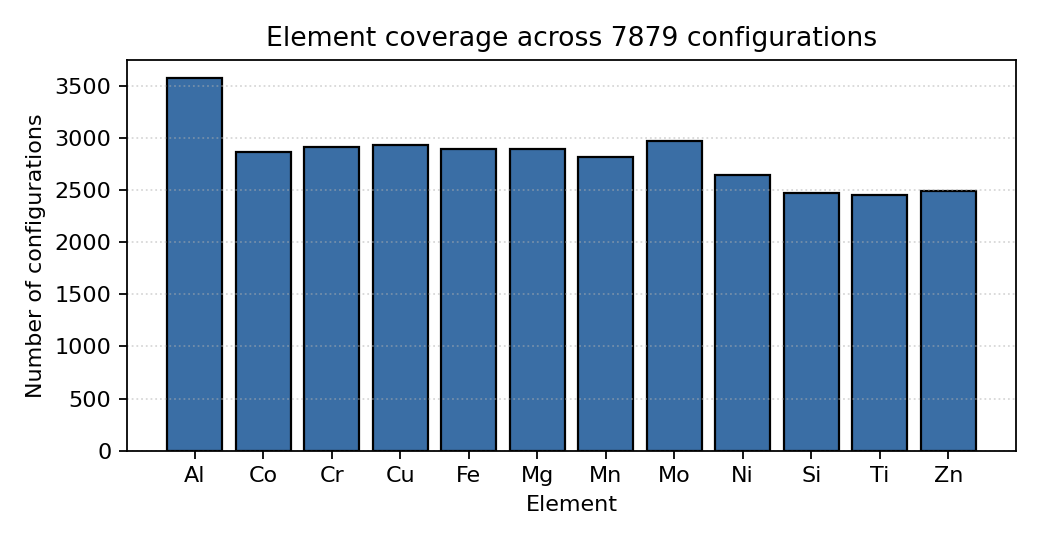
\includegraphics[width=0.98\linewidth]{figures/element_frequency.png}\\[-0.2em]
\scriptsize Element-occurrence distribution over the full
generated corpus.
\end{columns}
\end{frame}

% =====================================================================
% Slide 10: Stage 2 -- LAMMPS framework
% =====================================================================
\begin{frame}{Stage 2: The LAMMPS Framework}
\textbf{LAMMPS}~\citep{thompson2022}\footnote{\tiny LAMMPS = Large-scale Atomic/Molecular Massively Parallel Simulator (Sandia/Temple/NIST).}
is the de-facto MD code in materials science: classical
force-field integration on millions of atoms, MPI + OpenMP +
GPU parallelism, scripted via an in-process Python API.

\medskip
\begin{columns}[T]
\column{0.50\textwidth}
\textbf{Why a custom LAMMPS build was necessary.}
The upstream distribution caps the number of MEAM species at five,
which is incompatible with the 12-element library produced in
Stage~4. The species ceiling was therefore raised to twenty and a
private build of the shared library installed alongside the
standard tooling --- \emph{without this step the entire pipeline
is blocked on the first configuration containing more than five
distinct elements}.

\column{0.49\textwidth}
\begin{block}{Elastic protocol per configuration}
\small
\begin{enumerate}\itemsep0.15em
  \item Build $\sim\!4$\,nm cubic supercell from dominant element's
        lattice and composition-weighted $a_0$.
  \item Stochastically reassign atom types to match the requested
        composition.
  \item Anisotropic minimisation (cell + positions).
  \item Record baseline $\sigma_{xx},\sigma_{yy},\sigma_{zz}$.
  \item Apply $\delta = 10^{-3}$ axial strain
        $(\pm x,\pm y,\pm z)$, re-minimise, record stress.
  \item Central-difference $\to C_{11}\!\times\!3$,
        $C_{12}\!\times\!6$. Voigt average~\citep{voigt}.
\end{enumerate}
\end{block}
\end{columns}
\end{frame}

% =====================================================================
% Slide 11: Stage 2 -- MD results
% =====================================================================
\begin{frame}{Stage 2: MD Results across $\sim\!7800$ Alloys}
\centering
\scriptsize
\begin{tabular}{lrrrrrr}
\toprule
 Quantity   &    N &    Mean &   Median &   Std. &   Min &     Max \\
\midrule
 $E$ (GPa)  & 7815 & 132.88 &  103.61 & 69.10 & 3.07 & 398.31 \\
 $\nu$      & 7815 &   0.319 &    0.326 &  0.063 & 0.011 &   0.497 \\
\bottomrule
\end{tabular}\\[0.1em]
\textit{\scriptsize Dataset statistics after the
$0<E<400$\,GPa, $0<\nu<0.5$ physicality filter.}

\vspace{0.2em}
\begin{columns}[T]
\column{0.50\textwidth}
\centering
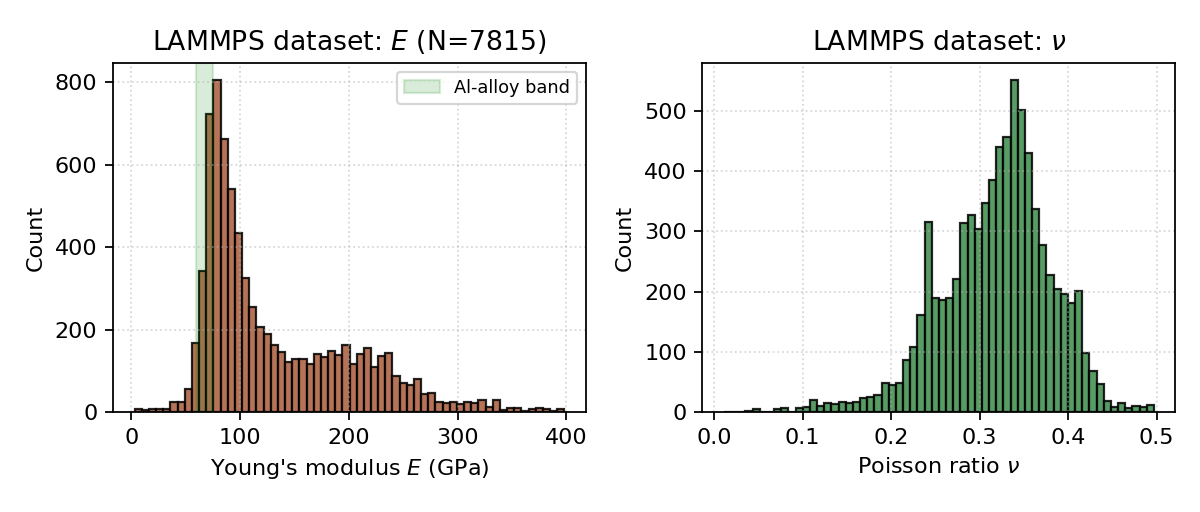
\includegraphics[width=0.99\linewidth]{figures/dataset_distributions.png}\\[-0.2em]
\scriptsize Histograms of $E$ (left) and $\nu$ (right).
Green band marks the $60\!-\!75$\,GPa Al-alloy range.

\column{0.49\textwidth}
\centering
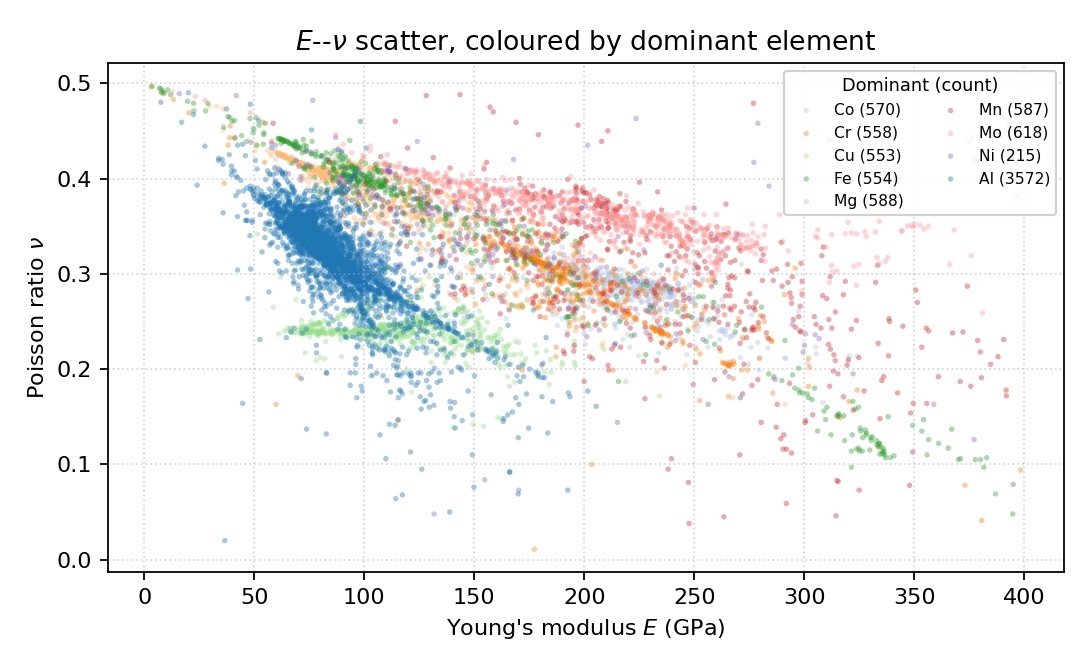
\includegraphics[width=0.92\linewidth]{figures/E_nu_scatter.png}\\[-0.2em]
\scriptsize $E$--$\nu$ scatter coloured by dominant element.
Refractory-rich (Mo, Cr, Fe) populate the high-$E$ wing.
\end{columns}
\end{frame}

% =====================================================================
% Slide 9: Stage 3-4 -- DFT references -> MEAM single-element init
% (Stage 4's alpha table dropped: its a0/Ecoh duplicate the table below)
% =====================================================================
\begin{frame}{Stage 3--4: DFT References $\to$ MEAM Initialisation}
\begin{columns}[T]
\column{0.45\textwidth}
\centering
\scriptsize
\setlength{\tabcolsep}{4pt}
\renewcommand{\arraystretch}{0.95}
\begin{tabular}{llrrr}
\toprule
Element & Lat. & $a_{0}$ (\AA) & $E_{\mathrm{coh}}$ & $B$ (GPa) \\
\midrule
Al & FCC     & 4.047 & 3.611 &  77.5 \\
Cu & FCC     & 3.639 & 3.857 & 138.5 \\
Si & DIAMOND & 5.471 & 5.130 &  89.3 \\
Ti & HCP     & 2.915 & 6.284 & 114.5 \\
Zn & HCP     & 2.766 & 0.964 &  68.4 \\
Cr & BCC     & 2.848 & 3.964 & 213.1 \\
Fe & BCC     & 2.806 & 6.834 & 420.5 \\
Mg & HCP     & 3.177 & 1.483 &  47.8 \\
Mn & BCC     & 2.803 & 3.728 & 225.7 \\
Mo & BCC     & 3.169 &10.353 & 280.8 \\
\bottomrule
\end{tabular}\\[0.2em]
\textit{Elemental references}
($E_{\mathrm{coh}}$ in eV/atom; Birch--Murnaghan fits).

\column{0.54\textwidth}
\centering
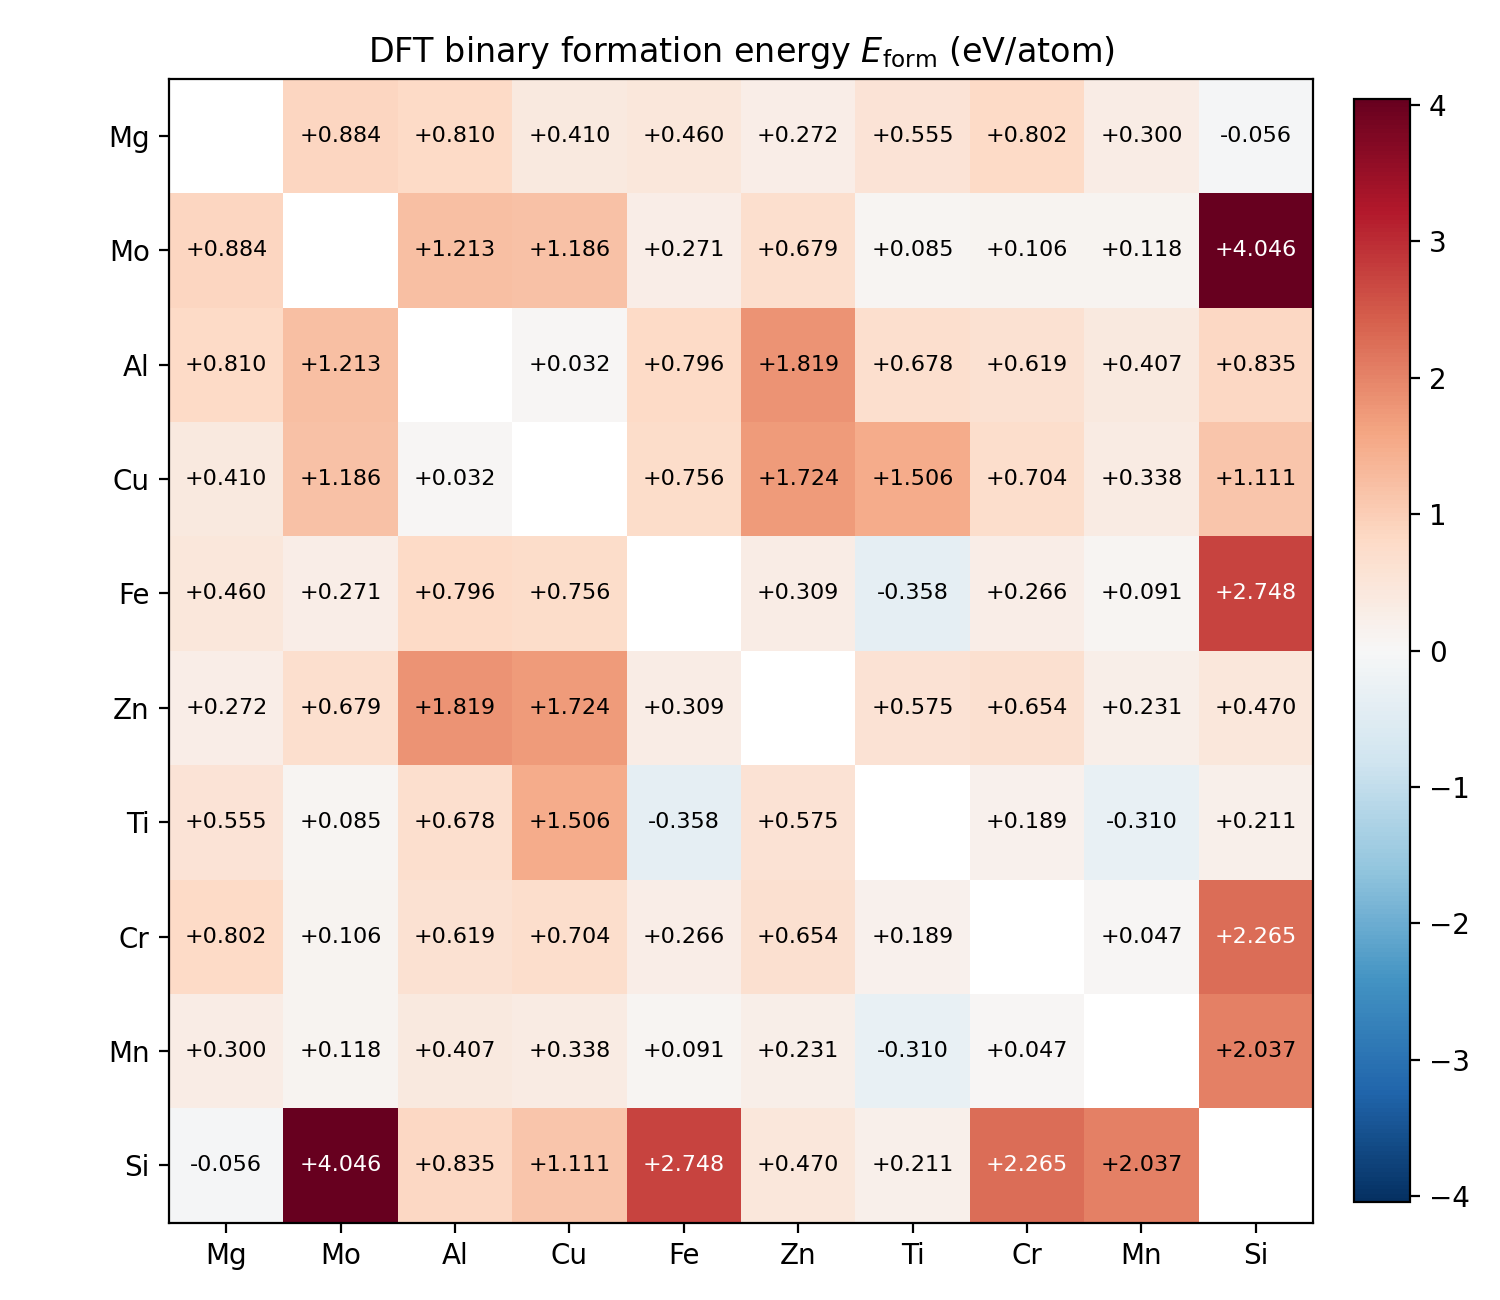
\includegraphics[height=3.7cm,keepaspectratio]{figures/formation_energy_heatmap.png}\\[-0.3em]
\scriptsize Binary formation energies $E_{\mathrm{form}}(i, j)$ (eV/atom):
negative $=$ exothermic mixing, positive $=$ limited solubility ---
these seed the MEAM cross-terms.

\smallskip
\begin{block}{Stage 4 --- single-element initialisation}
\scriptsize
Screening exponent from each DFT triple,\
$\alpha = a_{0}\sqrt{9 B \Omega / E_{\mathrm{coh}}}$
($\Omega$: cell volume)
$\to$ complete 12-element MEAM library ($\sim\!70$\,ms, cached).
$\alpha$-Mn EOS did not converge $\to$ relaxed-BCC approximation.
\end{block}
\end{columns}
\end{frame}
   % Stage 3--4 (DFT refs + MEAM init)
\input{slides/07_stage5a_composition_nn}
% =====================================================================
% Slide 12: Stage 5b -- NN-driven MEAM optimization
%   Left  : training process as bullets + Adam/Huber explained in body
%   Right : training-loss curve + result summary (histogram removed)
% =====================================================================
\begin{frame}{Stage 5b: NN-Driven MEAM Parameter Optimisation}
\fwtag{TensorFlow + LAMMPS}
\begin{columns}[T]
\column{0.5\textwidth}
\textbf{Closed-loop training process}
\begin{enumerate}\scriptsize
  \item \textbf{Surrogate.} A 4-layer MLP
        ($\to\!20\!\to\!20\!\to\!10\to$, ReLU) learns
        $(\text{MEAM params}) \to (C_{11}, C_{12})$.
  \item \textbf{Fit.} Trained with \emph{Adam}~\citep{kingma2015adam}
        on a \emph{Huber} loss ($\delta=1$), up to $10^{4}$ epochs,
        early-stopped once the loss falls below $5\!\times\!10^{-3}$.
  \item \textbf{Inverse step.} Adam (lr $0.01$, $3000$ steps) descends
        through the \emph{frozen} surrogate to the MEAM parameters that
        hit the target $(C_{11}, C_{12})$.
  \item \textbf{Loop.} Optimised parameters are re-evaluated in LAMMPS;
        new samples are appended and the surrogate retrained
        (active learning).
\end{enumerate}

\smallskip
\begin{block}{Why these choices}
\scriptsize
\textbf{Adam} --- adaptive-moment gradient optimiser: per-parameter step
sizes from running gradient moments, a robust default for NN training.\\
\textbf{Huber loss} --- squared-error for small residuals, absolute-error
for large ones; outlier configurations (Mg/Zn) cannot dominate the fit.
\end{block}

\column{0.5\textwidth}
\centering
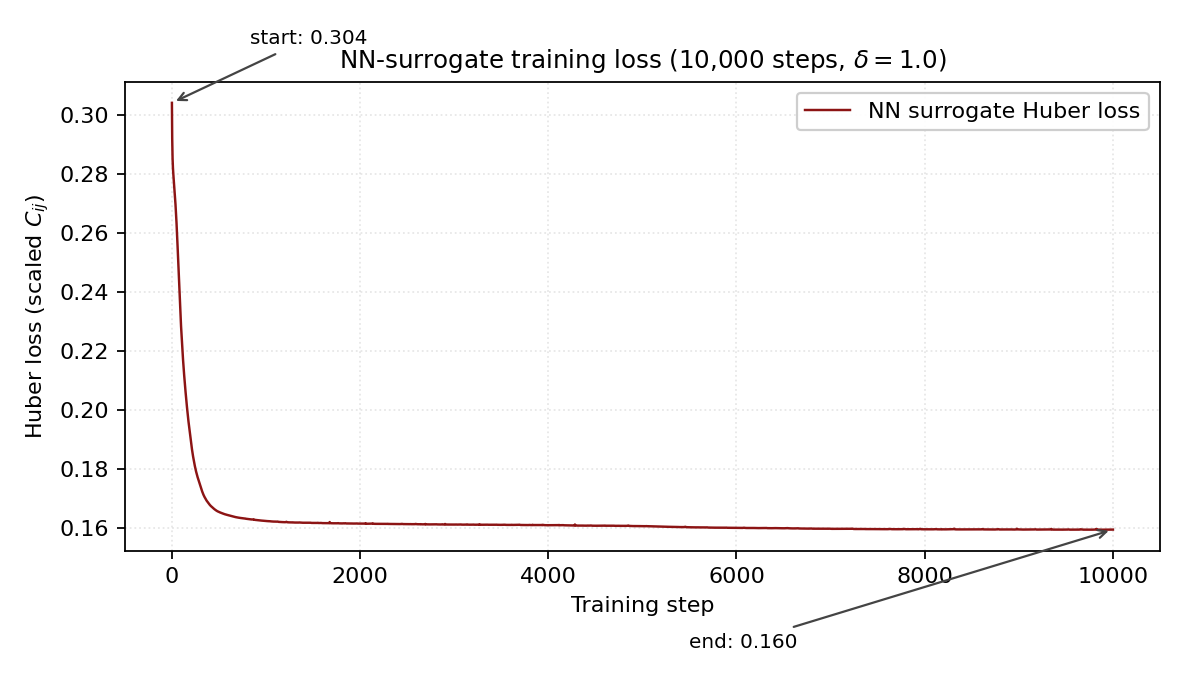
\includegraphics[width=0.74\linewidth]{figures/nnip_training_loss.png}\\[-0.4em]
\scriptsize Surrogate Huber-loss decays $1.0 \to 0.16$ over training.

\smallskip
\begin{block}{Result --- a working proof of concept}
\scriptsize
Tested on \textbf{30 unseen alloys}:
\begin{itemize}\scriptsize
  \item \textbf{11} gave a physically stable potential;
  \item \textbf{4} matched the MD reference within $\sim\!20\,\%$.
\end{itemize}
The pipeline runs end-to-end; accuracy grows with more data and
longer training (next slide).
\end{block}
\end{columns}
\end{frame}

% =====================================================================
% Slide 13: Summary -- what was achieved vs what comes next
% Two parallel columns reusing the deck badge language:
%   filled darkred check badge = done; outlined number badge = next.
% =====================================================================

% --- local badge / row / header helpers (slide-specific) -------------
\newcommand{\achbadge}{\tikz[baseline=-0.6ex]{\node[fill=darkred, text=white,
  rounded corners=2.5pt, minimum size=1.7em, inner sep=0pt,
  font=\small\bfseries]{\checkmark};}}
\newcommand{\nextbadge}[1]{\tikz[baseline=-0.6ex]{\node[draw=darkred,
  line width=0.7pt, text=darkred, rounded corners=2.5pt, minimum size=1.7em,
  inner sep=0pt, font=\small\bfseries]{#1};}}
\newcommand{\achrow}[1]{\smallskip\par\noindent
  \achbadge\hspace{0.7em}\parbox[t]{0.80\columnwidth}{\small #1}\par}
\newcommand{\nextrow}[2]{\smallskip\par\noindent
  \nextbadge{#1}\hspace{0.7em}\parbox[t]{0.80\columnwidth}{\small #2}\par}

\begin{frame}{Summary \& Further Studies}
\begin{columns}[T]

% ---------- achieved ----------
\column{0.49\textwidth}
{\tikz{\node[fill=darkred, text=white, rounded corners=3pt, inner sep=5pt,
  font=\bfseries\scshape]{Achieved};}}
\par\vspace{0.4em}
\achrow{\textbf{Automated 12-element MEAM pipeline.} An end-to-end
  workflow that assembles a multi-element potential.}
\achrow{\textbf{Aluminium-alloy elastic prediction.}
  $E,\nu$ and $C_{11},C_{12}$ obtained from composition.}
\achrow{\textbf{DFT-seeded, NN-trained MEAM.} First-principles
  references refit through a neural surrogate.}

% ---------- next ----------
\column{0.49\textwidth}
{\tikz{\node[draw=darkred, line width=0.7pt, text=darkred,
  rounded corners=3pt, inner sep=5pt, font=\bfseries\scshape]{What comes next};}}
\par\vspace{0.4em}
\nextrow{1}{\textbf{More data coverage.} Wider sampling across the
  composition space and crystal structures.}
\nextrow{2}{\textbf{More NN training epochs.} Deeper surrogate
  convergence before each refit.}
\nextrow{3}{\textbf{Denser atomic-cell DFT.} Finer cells and
  supercell sampling for sharper references.}
\nextrow{4}{\textbf{Inverse design.} Specify a target $(E, \nu)$ and
  invert the composition surrogate to propose candidate alloys.}

\end{columns}

\vspace{0.7em}
\centering{\footnotesize The pipeline already runs end to end; what is left is
more data, longer training, denser DFT references, and running the predictor
in reverse.}
\end{frame}

% =====================================================================
% Slide 23: References
% =====================================================================
\begin{frame}[allowframebreaks]{References}
\scriptsize
\setbeamertemplate{bibliography item}[text]
\renewcommand{\bibsection}{}
\bibliography{references}
\end{frame}


\end{document}
